\documentclass{csbeamer}

% Add custom packages
\usepackage{tikz}
\usetikzlibrary{calc, shapes.geometric, arrows.meta, positioning, arrows}
\usepackage{verbatim}
\usepackage{colortbl}
\usepackage{amsmath}
\usepackage{amssymb}
\usepackage{amsthm}

% Add custom color definitions
\definecolor{rlblue}{HTML}{1E88E5}
\definecolor{rlgreen}{HTML}{43A047}
\definecolor{rlred}{HTML}{E53935}
\definecolor{rlorange}{HTML}{FB8C00}
\definecolor{rlpurple}{HTML}{8E24AA}

% Course information
\university{St. Francis Xavier University}
\department{Department of Computer Science}
\course{CSCI-531 - Reinforcement Learning}
\courseshort{CSCI-531 - RL}
\term{Fall 2025}
\author{Dr. Jean-Alexis Delamer}

\title{Introduction to Reinforcement Learning}

\begin{document}

\frame{\titlepage}

% Section: What is Reinforcement Learning?
\section{What is Reinforcement Learning?}

\begin{frame}
    \frametitle{What is Reinforcement Learning (RL)?}
    \begin{itemize}
        \item<1-> Reinforcement learning is \textcolor{rlblue}{\textbf{what to do}} to \textcolor{rlorange}{\textbf{maximize a reward}}.
        \item<2-> We can give a more "formal" definition.
    \end{itemize}

    \only<3->{
        \begin{block}{Definition: Reinforcement Learning}
            Reinforcement Learning is calculating a function that maps \textcolor{rlblue}{\textbf{situations}} to \textcolor{rlgreen}{\textbf{actions}}.
        \end{block}
    }

    \only<4->{
        \begin{center}
            We said that we want to maximize a reward, but \textcolor{rlorange}{\textbf{what is a reward?}}
        \end{center}
    }
\end{frame}

\begin{frame}
    \frametitle{What is a Reward?}
    \begin{block}{Activity}
        \begin{center}
            \Large \textcolor{rlblue}{Try to explain what a reward is.}
        \end{center}
    \end{block}
\end{frame}

\begin{frame}
    \frametitle{Key Characteristics}
    \begin{itemize}
        \item<1-> To maximize a reward the learner can do \textcolor{rlgreen}{\textbf{different actions}}.
        \item<2-> If the learner was \textcolor{rlred}{\textbf{passive}}, it could not maximize anything.
        \item<3-> Usually, the learner starts with \textcolor{rlorange}{\textbf{no prior knowledge}} about what action it should do.
    \end{itemize}

    \only<4->{
        \begin{center}
            \Large \textcolor{rlblue}{What would you do to maximize a reward if you had no idea which action you should do?}
        \end{center}
    }
\end{frame}

\begin{frame}
    \frametitle{Strategy with No Knowledge}
    \begin{block}{Activity}
        \begin{center}
            \Large What would you do to maximize a reward if you had \textcolor{rlred}{\textbf{no idea}} which action you should do?
        \end{center}
    \end{block}

    \begin{center}
        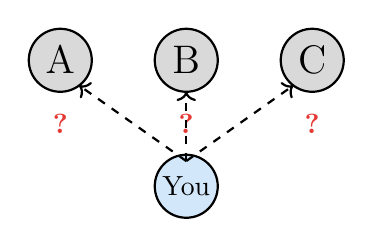
\begin{tikzpicture}[scale=0.8]
            % Unknown actions
            \foreach \x/\label in {0/A, 2/B, 4/C} {
                \draw[thick, fill=gray!30] (\x,1) circle (0.5);
                \node at (\x,1) {\Large \label};
                \node[below] at (\x,0.3) {\textcolor{rlred}{\textbf{?}}};
            }

            % Agent
            \draw[thick, fill=rlblue!20] (2,-1) circle (0.5);
            \node at (2,-1) {You};

            % Arrows to actions
            \draw[->, thick, dashed] (2,-0.6) -- (0.3,0.6);
            \draw[->, thick, dashed] (2,-0.6) -- (2,0.5);
            \draw[->, thick, dashed] (2,-0.6) -- (3.7,0.6);
        \end{tikzpicture}
    \end{center}

\end{frame}

% Section: A Simple Example
\section{A Simple Example: Learning to Navigate}

\begin{frame}
    \frametitle{A Simple Example: Learning to Navigate}
    \begin{block}{Scenario}
        \textbf{Imagine you're in a new city trying to find the best coffee shop.}
    \end{block}

    \begin{columns}
        \begin{column}{0.6\textwidth}
            \begin{itemize}
                \item<1-> \textbf{\textcolor{rlblue}{Your goal:}} Find great coffee (maximize reward)
                \item<2-> \textbf{\textcolor{rlgreen}{Your actions:}} Choose which direction to walk, which shops to try
                \item<3-> \textbf{\textcolor{rlorange}{Your feedback:}} Coffee quality (immediate), but also learning about the neighborhood (delayed)
                \item<4-> \textbf{\textcolor{rlred}{The challenge:}} Balance trying new places vs. returning to known good ones
            \end{itemize}
        \end{column}

        \begin{column}{0.4\textwidth}
            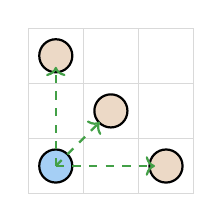
\begin{tikzpicture}[scale=0.7]
                % City grid
                \draw[thin, gray!30] (0,0) grid (3,3);

                % Coffee shops
                \visible<1->{
                    \foreach \x/\y in {0.5/2.5, 1.5/1.5, 2.5/0.5} {
                        \draw[thick, fill=brown!30] (\x,\y) circle (0.3);
                    }
                }

                % You
                \visible<1->{
                    \draw[thick, fill=rlblue!40] (0.5,0.5) circle (0.3);
                }

                % Exploration paths
                \visible<2->{
                    \draw[->, thick, dashed, rlgreen] (0.5,0.5) -- (0.5,2.3);
                    \draw[->, thick, dashed, rlgreen] (0.5,0.5) -- (1.3,1.3);
                    \draw[->, thick, dashed, rlgreen] (0.5,0.5) -- (2.3,0.5);
                }
            \end{tikzpicture}
        \end{column}
    \end{columns}

    \only<5->{
        \begin{center}
            \textit{This captures the essence of reinforcement learning!}
        \end{center}
    }
\end{frame}

\begin{frame}
    \frametitle{Coffee Shop Essence of RL}
    \begin{block}{This captures the essence of reinforcement learning:}
        \begin{enumerate}
            \item<1-> You have a \textcolor{rlblue}{\textbf{goal}} (good coffee)
            \item<2-> You take \textcolor{rlgreen}{\textbf{actions}} (choose directions/shops)
            \item<3-> You get \textcolor{rlorange}{\textbf{feedback}} (coffee quality)
            \item<4-> You \textcolor{rlpurple}{\textbf{learn and improve}} your strategy over time
            \item<5-> You must balance \textcolor{rlred}{\textbf{exploration}} (new places) vs \textcolor{rlblue}{\textbf{exploitation}} (known good places)
        \end{enumerate}
    \end{block}

    \only<6->{
        \begin{center}
            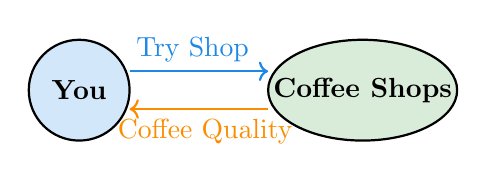
\begin{tikzpicture}[scale=0.8]
                % Simple RL loop
                \draw[thick, fill=rlblue!20] (0,0) circle (0.8);
                \node at (0,0) {\textbf{You}};

                \draw[thick, fill=rlgreen!20] (4.5,0) ellipse (1.5 and 0.8);
                \node at (4.5,0) {\textbf{Coffee Shops}};

                \draw[->, thick, rlblue] (0.8,0.3) -- (3,0.3);
                \node[above] at (1.8,0.3) {\textcolor{rlblue}{Try Shop}};

                \draw[->, thick, rlorange] (3,-0.3) -- (0.8,-0.3);
                \node[below] at (2,-0.3) {\textcolor{rlorange}{Coffee Quality}};
            \end{tikzpicture}
        \end{center}
    }
\end{frame}

\begin{frame}
    \frametitle{Coffee Shop Strategies}
    \begin{block}{Activity}
        In the coffee shop example:
    \end{block}

    \begin{enumerate}
        \item<1-> What would happen if you only went to the \textcolor{rlblue}{\textbf{first decent shop}} you found?
        \pause
        \item<2-> What would happen if you tried a \textcolor{rlorange}{\textbf{completely new shop every single day}}?
        \pause
        \item<3-> What's a \textcolor{rlgreen}{\textbf{good strategy for the long term}}?
    \end{enumerate}

    \only<4->{
        \begin{center}
            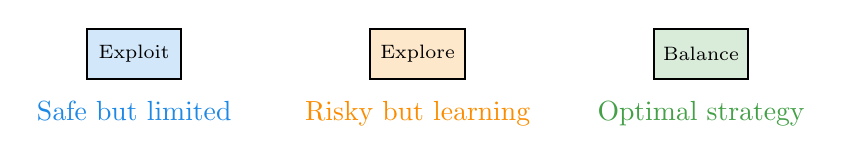
\begin{tikzpicture}[scale=0.8]
                % Strategy visualization
                \draw[thick, fill=rlblue!20] (-1,1) rectangle (0.5,1.8);
                \node at (-0.25,1.4) {\scriptsize Exploit};
                \node[below] at (-0.25,0.8) {\textcolor{rlblue}{Safe but limited}};

                \draw[thick, fill=rlorange!20] (3.5,1) rectangle (5,1.8);
                \node at (4.25,1.4) {\scriptsize Explore};
                \node[below] at (4.25,0.8) {\textcolor{rlorange}{Risky but learning}};

                \draw[thick, fill=rlgreen!20] (8,1) rectangle (9.5,1.8);
                \node at (8.75,1.4) {\scriptsize Balance};
                \node[below] at (8.75,0.8) {\textcolor{rlgreen}{Optimal strategy}};
            \end{tikzpicture}
        \end{center}
    }
\end{frame}

% Section: Key Concepts
\section{Key Concepts - The Basics}

\begin{frame}
    \frametitle{Key Concepts - The Basics}
    \begin{block}{Reinforcement learning has two main characteristics:}
        \begin{itemize}
            \item<1-> \textbf{\textcolor{rlblue}{Trial-and-error search:}} Learning by trying things and seeing what works
            \item<2-> \textbf{\textcolor{rlorange}{Delayed rewards:}} Actions now may have consequences much later
        \end{itemize}
    \end{block}

    \begin{columns}
        \begin{column}{0.5\textwidth}
            \only<1>{
                \begin{center}
                    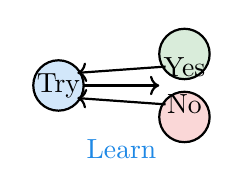
\begin{tikzpicture}[scale=0.8]
                        % Trial and error cycle
                        \draw[thick, fill=rlblue!20] (0,1) circle (0.4);
                        \node at (0,1) {Try};

                        \draw[->, thick] (0.4,1) -- (1.6,1);

                        \draw[thick, fill=rlgreen!20] (2,1.5) circle (0.4);
                        \node at (2,1.3) {Yes};

                        \draw[thick, fill=rlred!20] (2,0.5) circle (0.4);
                        \node at (2,0.7) {No};

                        \draw[->, thick] (1.7,1.3) -- (0.3,1.2);
                        \draw[->, thick] (1.7,0.7) -- (0.3,0.8);

                        \node[below] at (1,0.3) {\textcolor{rlblue}{Learn}};
                    \end{tikzpicture}
                \end{center}
            }
            \only<2>{
                \begin{center}
                    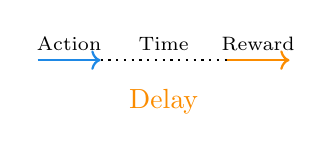
\begin{tikzpicture}[scale=0.8]
                        % Delayed reward timeline
                        \draw[->, thick, rlblue] (0,0) -- (1,0);
                        \node[above] at (0.5,0) {\scriptsize Action};

                        \draw[thick, dotted] (1,0) -- (3,0);
                        \node[above] at (2,0) {\scriptsize Time};

                        \draw[->, thick, rlorange] (3,0) -- (4,0);
                        \node[above] at (3.5,0) {\scriptsize Reward};

                        \node[below] at (2,-0.3) {\textcolor{rlorange}{Delay}};
                    \end{tikzpicture}
                \end{center}
            }
        \end{column}

        \begin{column}{0.5\textwidth}
            \textbf{Why these matter:}
            \begin{itemize}
                \item<1-> \textbf{Trial-and-error} means no teacher provides "correct" answers - you learn by experience
                \item<2-> \textbf{Delayed rewards} means you must connect actions to outcomes that happen later
            \end{itemize}
        \end{column}
    \end{columns}
\end{frame}

\begin{frame}
    \frametitle{Important Distinction}
    \begin{block}{Warning}
        Reinforcement learning is a name that regroups different concepts:
        \begin{itemize}
            \item<1-> It's a \textcolor{rlblue}{\textbf{type of problem}}.
            \item<2-> It's also a \textcolor{rlgreen}{\textbf{class of solution methods}}.
            \item<3-> And it's the \textcolor{rlorange}{\textbf{field}} that studies the two previous points as well.
        \end{itemize}
    \end{block}

    \only<4->{
        \begin{center}
            \Large \textcolor{rlred}{\textbf{You need to understand the distinction.}}
        \end{center}
    }
\end{frame}

% Section: The RL Problem
\section{What is the Reinforcement Learning Problem?}

\begin{frame}
    \frametitle{What is the Reinforcement Learning Problem? (Simplified)}
    \begin{itemize}
        \item<1-> The reinforcement learning problem is an idea coming from \textcolor{rlblue}{\textbf{dynamical system theory}}.
        \item<2-> And more specifically from the \textcolor{rlgreen}{\textbf{Markov Decision Processes}}.
        \item<3-> The basic ideas are:
        \begin{itemize}
            \item<4-> A learning agent must \textcolor{rlorange}{\textbf{sense}} the state of the environment.
            \item<5-> The agent must be able to take \textcolor{rlpurple}{\textbf{actions}} that affect the state.
            \item<6-> It must have a \textcolor{rlred}{\textbf{goal}} or goals relating to the state of the environment.
        \end{itemize}
    \end{itemize}

    \only<7->{
        \begin{center}
            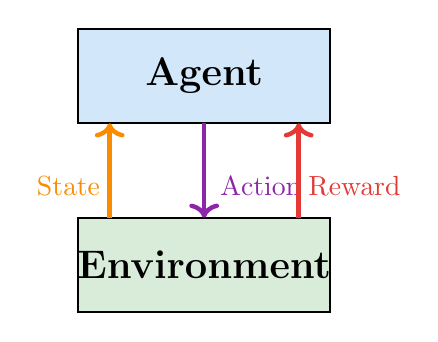
\begin{tikzpicture}[scale=0.8]
                % Agent box
                \draw[thick, fill=rlblue!20] (-2,-0.5) rectangle (2,1);
                \node at (0,0.25) {\Large \textbf{Agent}};

                % Environment box
                \draw[thick, fill=rlgreen!20] (-2,-3.5) rectangle (2,-2);
                \node at (0,-2.75) {\Large \textbf{Environment}};

                % Action arrow
                \draw[->, ultra thick, rlpurple] (0,-0.5) -- (0,-2);
                \node[right] at (0.1,-1.5) {\textcolor{rlpurple}{Action}};

                % State and reward arrows
                \draw[->, ultra thick, rlorange] (-1.5,-2) -- (-1.5,-0.5);
                \node[left] at (-1.5,-1.5) {\textcolor{rlorange}{State}};

                \draw[->, ultra thick, rlred] (1.5,-2) -- (1.5,-0.5);
                \node[right] at (1.5,-1.5) {\textcolor{rlred}{Reward}};
            \end{tikzpicture}
        \end{center}
    }
\end{frame}

\begin{frame}
    \frametitle{Agent-Environment Loop}
    \begin{center}
        \textit{This simple agent-environment loop might look basic, but it powers some of the most impressive AI breakthroughs.}
    \end{center}

    \pause
    \begin{center}
        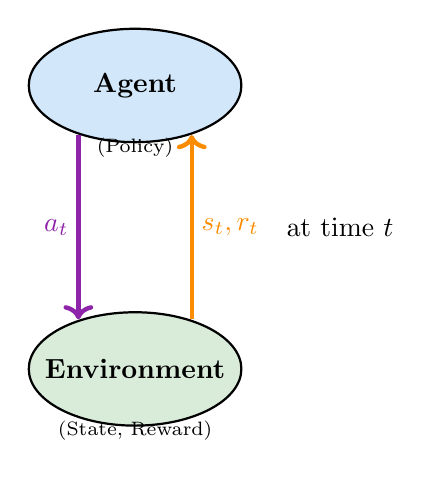
\begin{tikzpicture}[scale=0.9]
            % More detailed loop
            \draw[thick, fill=rlblue!20] (0,2) ellipse (1.5 and 0.8);
            \node at (0,2) {\textbf{Agent}};
            \node[below] at (0,1.4) {\scriptsize (Policy)};

            \draw[thick, fill=rlgreen!20] (0,-2) ellipse (1.5 and 0.8);
            \node at (0,-2) {\textbf{Environment}};
            \node[below] at (0,-2.6) {\scriptsize (State, Reward)};

            % Arrows with labels
            \draw[->, ultra thick, rlpurple] (-0.8,1.3) -- (-0.8,-1.3);
            \node[left] at (-0.8,0) {\textcolor{rlpurple}{$a_t$}};

            \draw[->, ultra thick, rlorange] (0.8,-1.3) -- (0.8,1.3);
            \node[right] at (0.8,0) {\textcolor{rlorange}{$s_t, r_t$}};

            % Time
            \node[right] at (2,0) {at time $t$};
        \end{tikzpicture}
    \end{center}
\end{frame}

% Section: Why RL Matters
\section{Why Reinforcement Learning Matters}

\begin{frame}
    \frametitle{Why Reinforcement Learning Matters}
    \begin{block}{Real-World Success Stories}
        \begin{itemize}
            \item<1-> \textbf{\textcolor{rlblue}{Game Playing:}} AlphaGo defeated world champions, mastering strategy through self-play
            \item<2-> \textbf{\textcolor{rlgreen}{Autonomous Systems:}} Self-driving cars make split-second decisions in complex environments
            \item<3-> \textbf{\textcolor{rlorange}{Finance \& Trading:}} Systems optimize investment decisions over time under uncertainty
        \end{itemize}
    \end{block}
\end{frame}

\begin{frame}
    \frametitle{What Makes These Problems Special?}
    \begin{block}{Why Traditional AI Approaches Fail}
        These problems require:
        \begin{enumerate}
            \item<1-> \textbf{Learning without a teacher} - no dataset of "perfect" decisions exists
            \item<2-> \textbf{Handling delayed consequences} - actions now affect outcomes much later
            \item<3-> \textbf{Adapting to change} - environment responds to your actions
            \item<4-> \textbf{Balancing exploration vs exploitation} - try new things vs use current knowledge
        \end{enumerate}
    \end{block}

    \only<5->{
        \begin{center}
            \textit{You might wonder: why couldn't traditional machine learning solve these problems? Understanding what RL is requires understanding what it's not.}
        \end{center}
    }
\end{frame}

% Section: What RL is NOT
\section{What Reinforcement Learning is NOT}

\begin{frame}
    \frametitle{What Reinforcement Learning is NOT?}
    \begin{block}{Understanding RL is easier when we compare it to other learning paradigms:}
    \end{block}

    \begin{center}
        \begin{tabular}{|l|c|c|c|}
            \hline
            \rowcolor{rlblue!20} \textbf{Learning Type} & \textbf{Data Required} & \textbf{Feedback Type} & \textbf{Goal} \\
            \hline
            \textbf{Supervised} & Labeled examples & Immediate correct answers & Predict/classify \\
            \hline
            \textbf{Unsupervised} & Unlabeled data & No feedback & Find patterns \\
            \hline
            \rowcolor{rlgreen!20} \textbf{Reinforcement} & Environment interaction & Delayed rewards & Maximize reward \\
            \hline
        \end{tabular}
    \end{center}

    \pause
    \begin{columns}
        \begin{column}{0.5\textwidth}
            \textbf{Example:} Email spam detection
            \begin{itemize}
                \item<2-> Has labeled data
                \item<3-> Immediate "correct" classification
                \item<4-> \textcolor{rlblue}{$\rightarrow$ Supervised Learning}
            \end{itemize}
        \end{column}

        \begin{column}{0.5\textwidth}
            \textbf{Example:} Game playing
            \begin{itemize}
                \item<5-> No "correct" move dataset
                \item<6-> Delayed consequences
                \item<7-> \textcolor{rlgreen}{$\rightarrow$ Reinforcement Learning}
            \end{itemize}
        \end{column}
    \end{columns}
\end{frame}

\begin{frame}
    \frametitle{Key Differences Explained}
    \begin{block}{Why supervised learning fails for RL problems:}
        \begin{itemize}
            \item<1-> \textbf{\textcolor{rlblue}{No perfect dataset:}} There's no collection of "correct" actions for every situation
            \item<2-> \textbf{\textcolor{rlgreen}{Context dependency:}} The best action depends on long-term consequences, not just current state
            \item<3-> \textbf{\textcolor{rlorange}{Interactive nature:}} The environment changes based on your actions
        \end{itemize}
    \end{block}

    \begin{block}{Why unsupervised learning isn't enough:}
        \begin{itemize}
            \item<4-> \textbf{\textcolor{rlred}{No objective:}} Finding patterns doesn't tell you which actions are good
            \item<5-> \textbf{\textcolor{rlpurple}{No feedback:}} You can't improve without knowing if you're doing well
        \end{itemize}
    \end{block}
\end{frame}

\begin{frame}
    \frametitle{Learning Paradigms}


    \begin{enumerate}
        \item<1-> Why can't you use supervised learning to learn chess strategy?
        \pause
        \item<2-> What would unsupervised learning find in a chess game, and why isn't that sufficient?
        \pause
        \item<3-> Give an example of a problem where you'd need each type of learning.
    \end{enumerate}
\end{frame}

% Section: Challenges
\section{The Challenges of Reinforcement Learning}

\begin{frame}
    \frametitle{The Challenges of Reinforcement Learning}
    \begin{block}{Reinforcement learning faces unique challenges that make it different from other machine learning approaches:}
    \end{block}

    \begin{center}
        \large {\textbf{The Exploration-Exploitation Trade-off}}
    \end{center}

    \pause
    \begin{center}
        \textit{This is the fundamental challenge in RL}
    \end{center}
\end{frame}

\begin{frame}
    \frametitle{The Exploration-Exploitation Trade-off}
    \begin{center}
        \begin{tabular}{|l|l|l|l|}
            \hline
            \rowcolor{rlblue!20} \textbf{Strategy} & \textbf{Description} & \textbf{Pros} & \textbf{Cons} \\
            \hline
            \textbf{Exploitation} & Use current knowledge & Immediate gains & Miss better options \\
            \hline
            \textbf{Exploration} & Try new actions & Discover better options & Short-term costs \\
            \hline
            \textbf{Balance} & Mix both strategies & Long-term optimal & Complex to implement \\
            \hline
        \end{tabular}
    \end{center}

    \pause
    \textbf{Examples:}
    \begin{itemize}
        \item<2-> \textbf{Exploitation:} Always go to your favorite restaurant
        \item<3-> \textbf{Exploration:} Try a new restaurant (might be bad)
        \item<4-> \textbf{Balance:} Sometimes try new places, sometimes stick to favorites
    \end{itemize}
\end{frame}

% \begin{frame}
%     \frametitle{Agent Decision Process}
%     \begin{center}
%         \begin{tikzpicture}[scale=1.0]
%             % Decision tree structure
%             \node[draw, fill=rlblue!20] (agent) at (0,3) {Agent faces decision};

%             \node[draw, fill=rlgreen!20] (actionA) at (-2,1.5) {Action A: Known good reward};
%             \node[draw, fill=rlorange!20] (actionB) at (2,1.5) {Action B: Unknown reward};

%             \draw[->, thick] (agent) -- (actionA);
%             \draw[->, thick] (agent) -- (actionB);

%             \node[below] at (-2,1) {\textcolor{rlgreen}{(reliable)}};
%             \node[below] at (2,1) {\textcolor{rlorange}{(risky)}};

%             % Strategies
%             \node[draw, fill=rlblue!20] (exploit) at (-2,0) {EXPLOIT: Choose A};
%             \node[draw, fill=rlorange!20] (explore) at (2,0) {EXPLORE: Try B};

%             \draw[->, thick] (actionA) -- (exploit);
%             \draw[->, thick] (actionB) -- (explore);

%             % Outcomes
%             \node[below] at (-2,-0.5) {\scriptsize Get expected reward};
%             \node[below] at (-2,-0.8) {\scriptsize (but miss learning)};

%             \node[below] at (2,-0.5) {\scriptsize Learn about B};
%             \node[below] at (2,-0.8) {\scriptsize (might find better option)};
%         \end{tikzpicture}
%     \end{center}

%     \only<2->{
%         \begin{center}
%             \textcolor{rlred}{\textbf{Key insight:}} You can't do only one strategy - pure exploitation gets stuck in local optima, pure exploration never uses what you learn.
%         \end{center}
%     }
% \end{frame}

% \begin{frame}
%     \frametitle{Activity: Personal Exploration-Exploitation}
%     \begin{block}{Interactive Activity}
%         Think of a time when you had to balance exploration vs exploitation in real life. How did you decide when to try something new vs stick with what you know?
%     \end{block}

%     \pause
%     \textbf{Examples might include:}
%     \begin{itemize}
%         \item<2-> Choosing restaurants
%         \item<3-> Picking courses/majors
%         \item<4-> Job searching
%         \item<5-> Investment decisions
%     \end{itemize}

%     \only<6->{
%         \begin{center}
%             \textcolor{rlgreen}{\textbf{Share your example with a neighbor!}}
%         \end{center}
%     }
% \end{frame}

\begin{frame}
    \frametitle{The Whole Problem Challenge}
    \begin{block}{The Whole Problem Challenge}
        \begin{itemize}
            \item<1-> \textbf{\textcolor{rlblue}{Complete system:}} RL considers the entire problem from start to finish
            \item<2-> \textbf{\textcolor{rlgreen}{Goal-seeking agent:}} Must actively pursue objectives, not just respond to inputs
            \item<3-> \textbf{\textcolor{rlorange}{Uncertainty handling:}} Must operate effectively despite incomplete information about the environment
        \end{itemize}
    \end{block}

    \only<4->{
        \begin{center}
            \textit{Understanding these challenges prepares us to examine what makes RL systems work. Every RL agent relies on the same core building blocks.}
        \end{center}
    }
\end{frame}

% Section: Elements of RL
\section{Elements of Reinforcement Learning}

% \begin{frame}
%     \frametitle{Elements of Reinforcement Learning}
%     \begin{block}{Every RL system consists of four key components that work together:}
%     \end{block}

%     \pause
%     \begin{center}
%         \Large \textcolor{rlblue}{What are the two elements we talked about that compose reinforcement learning?}
%     \end{center}

%     \pause
%     \begin{center}
%         \textcolor{rlgreen}{\textbf{Think about it for 30 seconds...}}
%     \end{center}
% \end{frame}

% \begin{frame}
%     \frametitle{Activity: Elements Review}
%     \begin{block}{Interactive Activity}
%         What are the two elements we talked about that compose reinforcement learning?
%     \end{block}

%     \pause
%     \begin{center}
%         \begin{tikzpicture}[scale=0.8]
%             % Two empty boxes
%             \draw[thick, fill=gray!20] (0,1) rectangle (2,2);
%             \node at (1,1.5) {\Large 1. ?};

%             \draw[thick, fill=gray!20] (3,1) rectangle (5,2);
%             \node at (4,1.5) {\Large 2. ?};
%         \end{tikzpicture}
%     \end{center}

%     \pause
%     \begin{center}
%         \textcolor{rlgreen}{\textbf{Hint: One was about learning by trying, one was about consequences over time...}}
%     \end{center}

%     \only<4->{
%         \begin{center}
%             \textcolor{rlblue}{\textbf{Answers:}} Trial-and-error search \& Delayed rewards
%         \end{center}
%     }
% \end{frame}

\begin{frame}
    \frametitle{The Four Core Elements}
    \begin{center}
        \begin{tabular}{|l|l|l|c|}
            \hline
            \rowcolor{rlblue!20} \textbf{Element} & \textbf{Purpose} & \textbf{Think of it as...} & \textbf{Required?} \\
            \hline
            \textbf{Policy} & Decision maker & The brain that chooses actions & Essential \\
            \hline
            \textbf{Reward Function} & Goal definition & The scoring system & Essential \\
            \hline
            \textbf{Value Function} & Long-term predictor & The strategic advisor & Essential \\
            \hline
            \textbf{Model} & Environment simulator & The crystal ball & Optional \\
            \hline
        \end{tabular}
    \end{center}

    \pause
    \begin{center}
        \textit{These four elements work together like a team - each has a specific role, but their real power comes from how they interact in the learning process.}
    \end{center}
\end{frame}

\begin{frame}
    \frametitle{1. Policy - The Decision Maker}
    \begin{block}{Definition: Policy}
        A policy is a function that maps each state to an action.
    \end{block}

    \begin{columns}
        \begin{column}{0.6\textwidth}
            \textbf{What it does:}
            \begin{itemize}
                \item<1-> Defines the behavior of an agent at any given time
                \item<2-> Core of the RL agent - determines all actions
                \item<3-> Can be deterministic (same action every time) or stochastic (probabilistic)
            \end{itemize}

            \only<4->{
                \textbf{Examples:}
                \begin{itemize}
                    \item \textbf{Chess:} "If opponent threatens my queen, move it to safety"
                    \item \textbf{Trading:} "If price drops 5\%, sell 20\% of holdings"
                    \item \textbf{Navigation:} "If obstacle ahead, turn left"
                \end{itemize}
            }
        \end{column}

        \begin{column}{0.4\textwidth}
            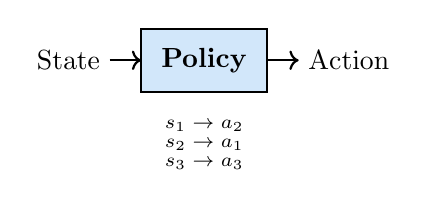
\begin{tikzpicture}[scale=0.8]
                % Policy function visualization
                \draw[thick, fill=rlblue!20] (0,1) rectangle (2,2);
                \node at (1,1.5) {\textbf{Policy}};

                % State input
                \draw[->, thick] (-0.5,1.5) -- (0,1.5);
                \node[left] at (-0.5,1.5) {State};

                % Action output
                \draw[->, thick] (2,1.5) -- (2.5,1.5);
                \node[right] at (2.5,1.5) {Action};

                % Examples
                \visible<4->{
                    \node[below] at (1,0.7) {\scriptsize $s_1 \rightarrow a_2$};
                    \node[below] at (1,0.4) {\scriptsize $s_2 \rightarrow a_1$};
                    \node[below] at (1,0.1) {\scriptsize $s_3 \rightarrow a_3$};
                }
            \end{tikzpicture}
        \end{column}
    \end{columns}
\end{frame}

\begin{frame}
    \frametitle{2. Reward Function - The Goal Definition}
    \begin{block}{Definition: Reward}
        A reward is a value returned by the environment at a time step $t$.
    \end{block}

    \textbf{What it does:}
    \begin{itemize}
        \item<1-> Defines the goal of the RL problem
        \item<2-> Provides immediate feedback for actions
        \item<3-> Agent's objective: maximize total reward over time
    \end{itemize}

    \only<4->{
        \textbf{Examples:}
        \begin{itemize}
            \item \textbf{Game:} +10 for winning, -1 for losing, 0 for draw
            \item \textbf{Robot:} +1 for forward movement, -10 for collision
            \item \textbf{Trading:} +profit for good trades, -loss for bad ones
        \end{itemize}
    }
\end{frame}

\begin{frame}
    \frametitle{3. Value Function - The Strategic Advisor}
    \begin{block}{Definition: Value Function}
        A value function is a function returning for each state the total expected reward starting from this state.
    \end{block}

    \textbf{What it does:}
    \begin{itemize}
        \item<1-> Estimates long-term expected reward from each state
        \item<2-> Helps agent think strategically, not just about immediate rewards
        \item<3-> Much harder to determine than immediate rewards
    \end{itemize}

    \only<4->{
        \begin{center}
            \textcolor{rlred}{\textbf{Key insight:}} We seek actions that lead to states with higher \textcolor{rlgreen}{\textbf{value}}, not higher immediate \textcolor{rlorange}{\textbf{reward}}.
        \end{center}
    }
\end{frame}

\begin{frame}
    \frametitle{Activity: Reward vs Value}
    \begin{block}{Interactive Activity}
        \textbf{Reward vs Value - Which would you choose?}
        \begin{itemize}
            \item State A: immediate reward = 100, long-term value = 3
            \item State B: immediate reward = 1, long-term value = 5
        \end{itemize}
    \end{block}

    \pause
    \begin{center}
        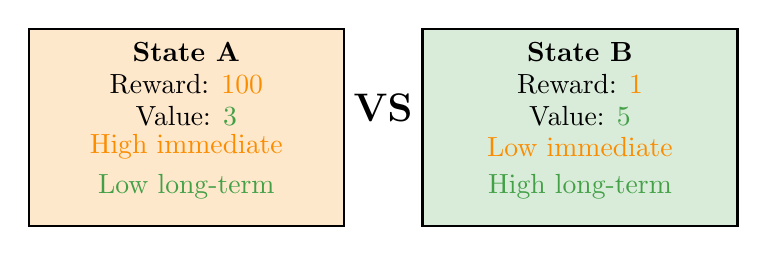
\begin{tikzpicture}[scale=1.0]
            % State A
            \draw[thick, fill=rlorange!20] (-2,-0.5) rectangle (2,2);
            \node at (0,1.7) {\textbf{State A}};
            \node at (0,1.3) {Reward: \textcolor{rlorange}{100}};
            \node at (0,0.9) {Value: \textcolor{rlgreen}{3}};
            \node at (0,0.5) {\textcolor{rlorange}{High immediate}};
            \node at (0,0) {\textcolor{rlgreen}{Low long-term}};

            % VS
            \node at (2.5,1) {\Large \textbf{VS}};

            % State B
            \draw[thick, fill=rlgreen!20] (3,-0.5) rectangle (7,2);
            \node at (5,1.7) {\textbf{State B}};
            \node at (5,1.3) {Reward: \textcolor{rlorange}{1}};
            \node at (5,0.9) {Value: \textcolor{rlgreen}{5}};
            \node at (5,0.5) {\textcolor{rlorange}{Low immediate}};
            \node at (5,0) {\textcolor{rlgreen}{High long-term}};
        \end{tikzpicture}
    \end{center}

    \pause
    \textcolor{rlblue}{\textbf{Question:}} Why might State B be better despite lower immediate reward?
\end{frame}

\begin{frame}
    \frametitle{Value vs Reward Examples}
    \textbf{Examples of choosing value over immediate reward:}
    \begin{itemize}
        \item<1-> \textbf{\textcolor{rlblue}{Chess:}} Sacrificing a piece (negative reward) to gain better position (higher value)

    \end{itemize}

    \only<4->{
        \begin{center}
            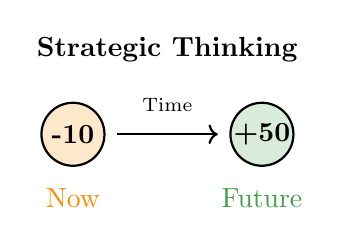
\begin{tikzpicture}[scale=0.8]
                % Immediate vs long-term visualization
                \draw[thick, fill=rlorange!20] (0,1) circle (0.5);
                \node at (0,1) {\textbf{-10}};
                \node[below] at (0,0.3) {\textcolor{rlorange}{Now}};

                \draw[->, thick] (0.7,1) -- (2.3,1);
                \node[above] at (1.5,1.2) {\scriptsize Time};

                \draw[thick, fill=rlgreen!20] (3,1) circle (0.5);
                \node at (3,1) {\textbf{+50}};
                \node[below] at (3,0.3) {\textcolor{rlgreen}{Future}};

                \node[above] at (1.5,2) {\textbf{Strategic Thinking}};
            \end{tikzpicture}
        \end{center}
    }
\end{frame}

\begin{frame}
    \frametitle{4. Model - The Crystal Ball (Optional)}
    \begin{block}{Definition: Model}
        The model of the environment is the representation of the dynamic of the problem.
    \end{block}

    \textbf{What it does:}
    \begin{itemize}
        \item<1-> Predicts what happens next: given current state and action, what's the next state and reward?
        \item<2-> Allows agent to plan ahead and simulate different strategies
        \item<3-> Not always available or practical to learn
    \end{itemize}

    \only<4->{
        \begin{center}
            \begin{tabular}{|l|c|l|l|}
                \hline
                \rowcolor{rlblue!20} \textbf{Type} & \textbf{Model?} & \textbf{Characteristics} & \textbf{Examples} \\
                \hline
                \textbf{Model-based} & Yes & Can plan ahead, simulate scenarios & Chess engines \\
                \hline
                \textbf{Model-free} & No & Learn directly from experience & Most game AI\\
                \hline
            \end{tabular}
        \end{center}
    }
\end{frame}

% Section: Summary
\section{Summary}

\begin{frame}
    \frametitle{Summary}
    \begin{block}{You now understand the core building blocks of reinforcement learning!}
        From our coffee shop example to these fundamental elements, you've seen how RL systems learn through experience.
    \end{block}

    \textbf{What we've covered:}
    \begin{itemize}
        \item<1-> \textbf{\textcolor{rlblue}{Core RL Concepts:}} Trial-and-error learning with delayed rewards
        \item<2-> \textbf{\textcolor{rlgreen}{Key Elements:}} Policy, rewards, values, and models
        \item<3-> \textbf{\textcolor{rlorange}{Main Challenge:}} Balancing exploration vs exploitation
        \item<4-> \textbf{\textcolor{rlpurple}{Why RL Matters:}} Real-world applications where traditional AI fails
    \end{itemize}

    \only<5->{
        \begin{center}
            \textcolor{rlred}{\textbf{Up Next: Multi-Armed Bandits}}
        \end{center}
    }
\end{frame}

\begin{frame}
    \frametitle{Current Limitations \& Assumptions}
    \begin{block}{RL is powerful but has important limitations to keep in mind:}
    \end{block}

    \begin{center}
        \begin{tabular}{|l|l|l|}
            \hline
            \rowcolor{rlblue!20} \textbf{Challenge} & \textbf{Description} & \textbf{Impact} \\
            \hline
            \textbf{State Design} & How to represent the current situation & Learning speed \\
            \hline
            \textbf{State Space Size} & Too many possible states & Learning speed \\
            \hline
            \textbf{Partial Observability} & Can't see everything relevant & Incomplete info \\
            \hline
        \end{tabular}
    \end{center}

    \textbf{Key Points:}
    \begin{itemize}
        \item<1-> \textbf{State is everything:} The quality of state representation determines learning success
        \item<2-> \textbf{Not magic:} RL assumes you can define reasonable states, actions, and rewards
        \item<3-> \textbf{Design matters:} How you frame the problem affects what the agent can learn
    \end{itemize}
\end{frame}

\begin{frame}
    \frametitle{Activity: Driving Example}
    \begin{block}{Interactive Activity}
        Think about teaching someone to drive:
    \end{block}

    \begin{enumerate}
        \item<1-> What information (state) do they need to make good decisions?
        \pause
        \item<2-> What if they could only see through a small window - how would this affect learning?
        \pause
        \item<3-> How would you define "good driving" as rewards?
    \end{enumerate}
\end{frame}

\end{document}
